\section{Telescope substitution: from Urania's tube to Skywatcher's tube}
Passing from the Urania telescope to Skywatcher telescope we have faced the problem of how to insert the latter in the telescope mount.
Indeed, since Skywatcher's telescope diameter is 200mm it does not fit inside the mount fork.

Our solution is to insert a seat in which to place the telescope.
The barycenter of the telescope is not centered with the DEC axis, thus we have settled a post capable of holding weights to balance the forces.
See figure \ref{fig:piastra_DEC} and \ref{fig:piastra_particular}.
\\
\begin{minipage}{0.25\textwidth}
    \centering
    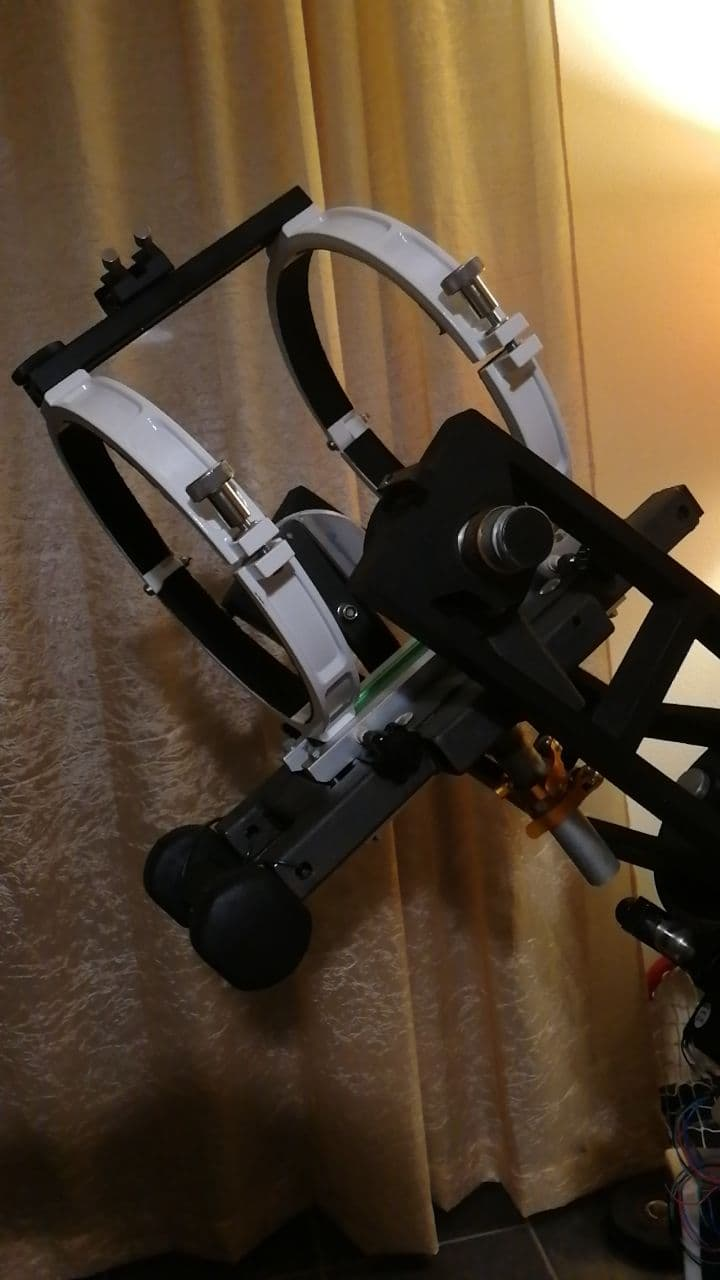
\includegraphics[scale=0.5]{DEC_sede.jpg}
    \captionof{figure}{The mechanism built to insert Skywatcher's telescope into the Urania robust mount.}
    \label{fig:piastra_DEC}
\end{minipage}
\begin{minipage}
    {0.25\textwidth}
    \centering
    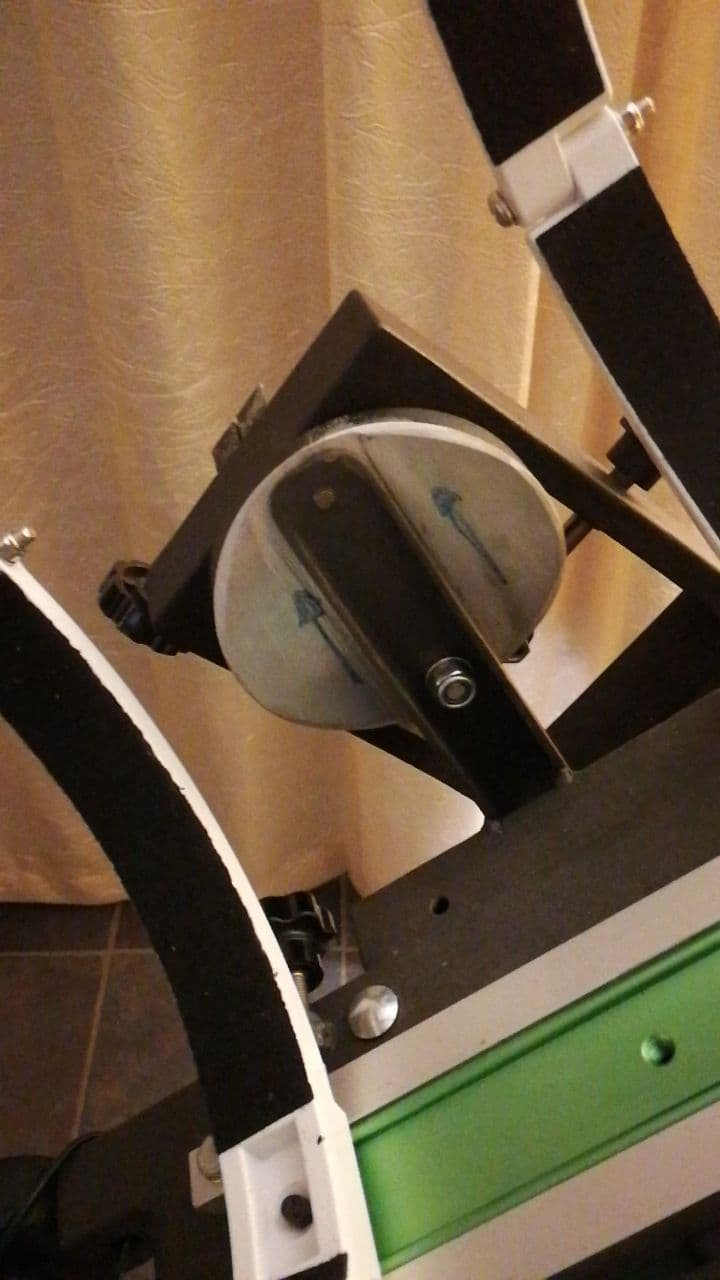
\includegraphics[scale=0.5]{DEC_piastra.jpg}
    \captionof{figure}{detail of the replacement plate that supports the new telescope.}
    \label{fig:piastra_particular}
\end{minipage}
\\
The scheme with distances is visible in figure \ref{fig:DEC_piastra_dimensioni}.
\\
\begin{minipage}
    {0.5\textwidth}
    \centering
    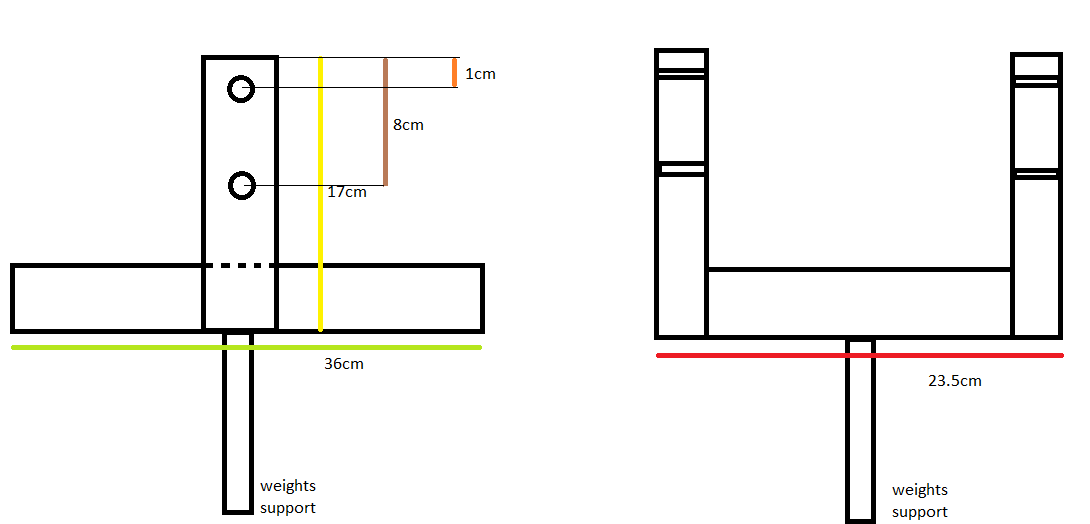
\includegraphics[scale=0.75]{DEC_piastra_dimensioni.png}
    \captionof{figure}{Schematic view of the telescope mount insertion.
    This represents only the installation build with some squared metal bars upon which the two white loops (which hold the telescope tube) are fixed and are not illustrated in this scheme. The two holes in each arm serve to fix the structure on the mount. }
    \label{fig:DEC_piastra_dimensioni}
\end{minipage}

Lastly, to enhance the fluidity of motion and reduce the backlash, the rotation mechanism is enriched with a system of two bearing for each fork arm, one interior and one fixed in the mount externally, see figure \ref{fig:cuscinetto-DEC}.
\\
\begin{minipage}
    {.5\textwidth}
    \centering
    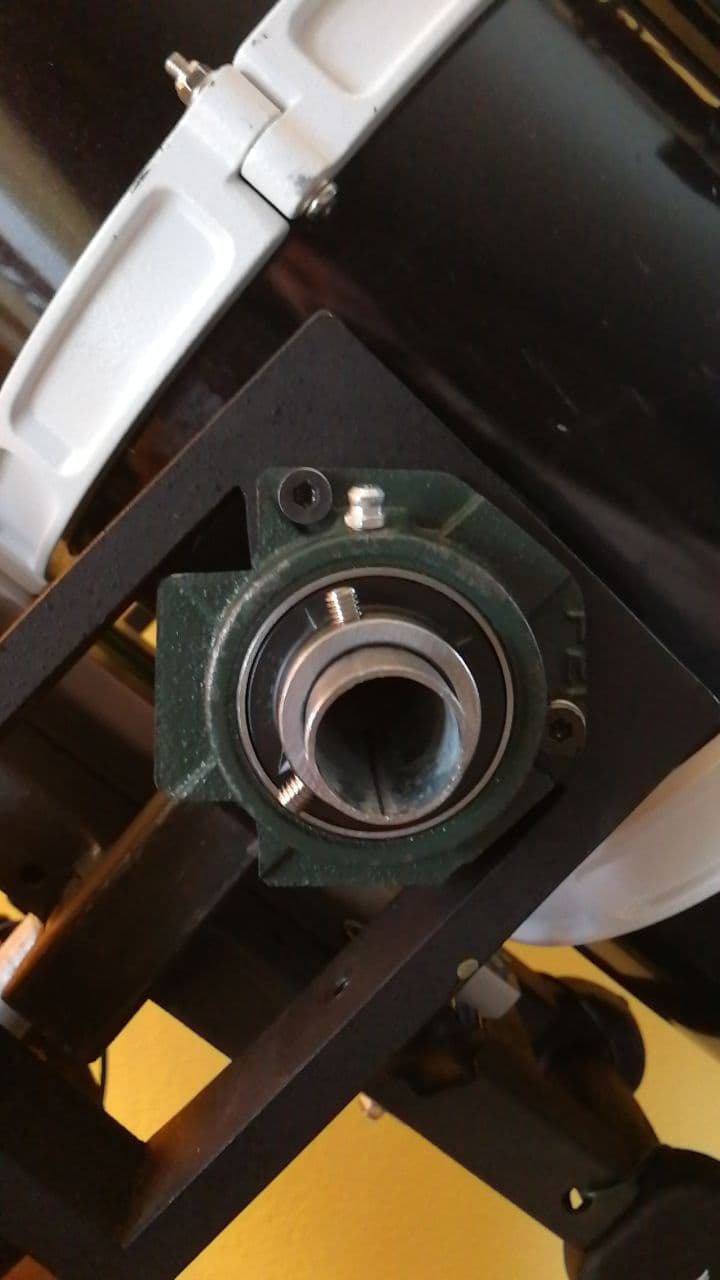
\includegraphics[scale=.45]{cuscinetto-dec.jpg}
    \captionof{figure}{External bearing mounted on one fork arm.}
    \label{fig:cuscinetto-DEC}
\end{minipage}